\chapter{相关技术}
在本章节我们介绍和讨论本论文的相关技术,包括流量加密、流量混淆、流量分析、Tor、TLS协议和SOCKS协议。

\section{流量加密}
流量加密是对抗流量分析的最常见手段,加密使加密的数据变得难以理解和分析。
为了保护互联网终端用户的隐私,客户端和服务器之间的加密通信正在成为常态。
例如随着HTTPS的广泛普及和使用,现在网络上的大部分HTTP流量都是通过TLS加密的流量,这保证了通信双方传输数据的加密性、认证性和完整性。
此外,为了提高最终用户的安全性和体验质量,出现了新的协议(例如HTTP/2和QUIC),它们克服了HTTP/1.1的各种限制。
但是,HTTP/2的新特性,例如有效载荷加密、多路复用和并发和服务器推送,增加了流量分析的复杂性。

\begin{figure}[H]
  \centering
  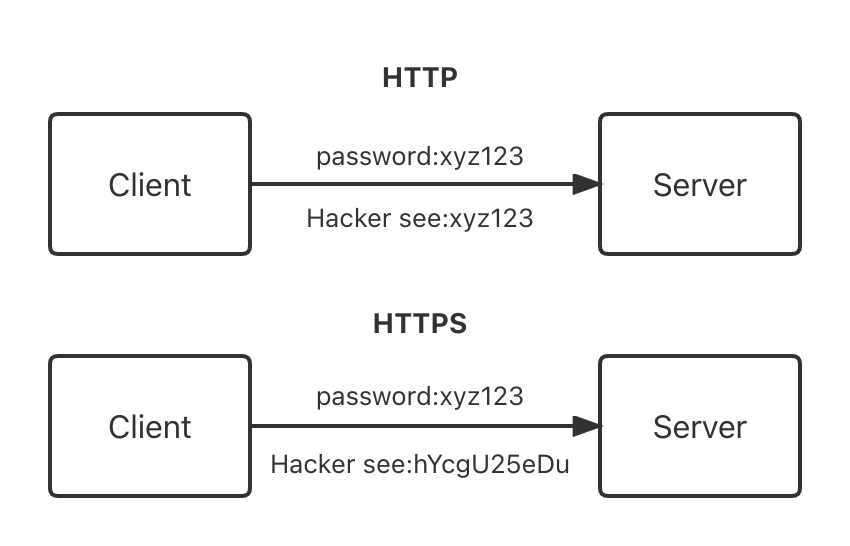
\includegraphics[width=\textwidth]{https}
  \caption{通过HTTPS,通信双方传输的数据得到加密,攻击者难以分析加密数据报文。}
\end{figure}

然而大多数加密协议的加密数据包有效负载中都包含标识协议的明文头,协议特征明显,能够被精准识别。
例如VPN协议WireGuard\cite{donenfeld2017wireguard}不支持流量混淆,基于其流量特征(使用端口号 51280、固定的消息长度(初始化/响应/cookie分别为148/92/64字节)、在初始化和响应消息的末尾有16个零字节),很容易分辨出在使用WireGuard协议加密数据。
这样,虽然攻击者不知道加密流量的具体明文内容,但可以识别出加密流量所使用的协议。


\section{流量混淆}
流量混淆是一种通过更改数据包(例如,在数据包中添加随机字节以增加数据包大小)来限制攻击者的信息收集的技术。
流量混淆可以有效地减少被动侦查的风险,即攻击者收集流量并使用统计分析来归类不同的模式(如流量协议,应用程序,用户信息等)。
这种技术的一个主要问题是在可行的修改和网络开销的限制下,确定有效掩盖流量特征的最佳算法。

第一种常用的方法是随机化,通过对原始流量的数据进行加密,数据包通过插入随机大小的载荷使其大小随机。
这种方法使得加密流量没有规律,数据报文内容和数据包大小都是随机的。
另一种常用的方法是模仿广泛使用的流量,比如HTTPS。
通过这种方法,攻击者难以将加密流量从普通的流量分辨出来,从而达到了流量混淆的目的。

\section{流量分析}
流量分析是一个完整的过程,从捕获流量数据开始,到发现互联网网络中的关系、模式、异常情况和错误配置等内容。
特别是,流量分类是该领域策略的一个子组,其目的是将互联网流量分为预先定义的类别,如正常或异常流量、应用程序的类型(流媒体、网页浏览、VoIP等)或应用程序的名称(YouTube、Netflix、Facebook等)。
网络流量分类是很重要的,因为涉及到以下几个原因:
\begin{enumerate}
  \item \textbf{故障排除任务}:主要目的是定位有故障的网络设备、设备/软件的错误配置、定位丢包点、网络错误等。 
  \item \textbf{安全}:通过对互联网流量进行分析,来避免恶意软件或防止私人信息被入侵。
  \item \textbf{服务质量(QoS)管理}:通过确保和完善服务质量,来提高最终用户对应用程序或服务的整体可接受性。在这个领域,识别或分类网络中的应用程序的名称或类型有助于预先处理一些方面。例如,从流量中识别不同的应用对于管理带宽资源和确保QoS要求至关重要。
\end{enumerate}

在过去,流量分类依赖于基于端口的方法,即每个应用程序通过其注册和已知的端口来识别,这些端口由互联网号码分配机构(IANA)定义。
这种方法逐渐变得不可靠和不准确,原因之一是具有未注册或随机生成的端口的新应用程序的扩散。
另一种在该领域获得大量普及的方法是深度包数据报文检测(DPI),DPI通过在数据包有效载荷和一组存储的签名之间进行匹配,对网络流量进行分类。
然而,当隐私政策和法律阻止访问数据包内容时,以及在流量协议混淆或封装的情况下,DPI会失败。

机器学习(ML)和深度学习(DL)无疑已经变得越来越有影响力,它们的应用已经扩展到广泛的领域,包括流量分析。
在过去的二十年里,大量的文献已经被提出,通过利用机器学习和深度学习技术,来实现不同的流量分类目标,如服务级分类(即分类为粗粒度的服务类别),例如服务级别分类(粗粒度服务类别,例如视频流、聊天和网络邮件)、应用级别分类(即细粒度类别,某一特定的应用程序),服务质量 (QoS) 级别和恶意流量检测。
基于ML和DL的流量分析展现出巨大的潜力,在许多具体的流量分类问题取得了很好的效果\cite{rezaei2019deep}。
然而,仍有各种限制需要解决,以使其在现实世界中得到实际应用。

\section{Tor}
Tor\cite{dingledine2004tor}是The Onion Router(洋葱路由器)的缩写,是一款免费的开源软件,用于实现匿名通信。
它通过一个由六千多个中继器组成的免费的、全球性的、志愿的覆盖网络来引导用户流量,以隐藏用户的位置和使用情况,使其不被任何进行网络监控或流量分析的人发现。
Tor通过在通信协议栈的应用层中对传输流量进行加密,来实现洋葱路由这一技术。
Tor会对包括下一个节点的IP地址在内的数据,进行多次加密,并通过虚拟电路(包括随机选择的Tor节点)将其提交。
每个中继节点都会对一层加密的数据进行解密,以知道加密数据的下一个发送目的地,然后将剩余的加密数据发送给它。
最后的中继节点会解密最内层的加密数据,并在不会泄露或得知源IP地址的情况下,将原始数据发送至目标地址。

\begin{figure}[H]
  \centering
  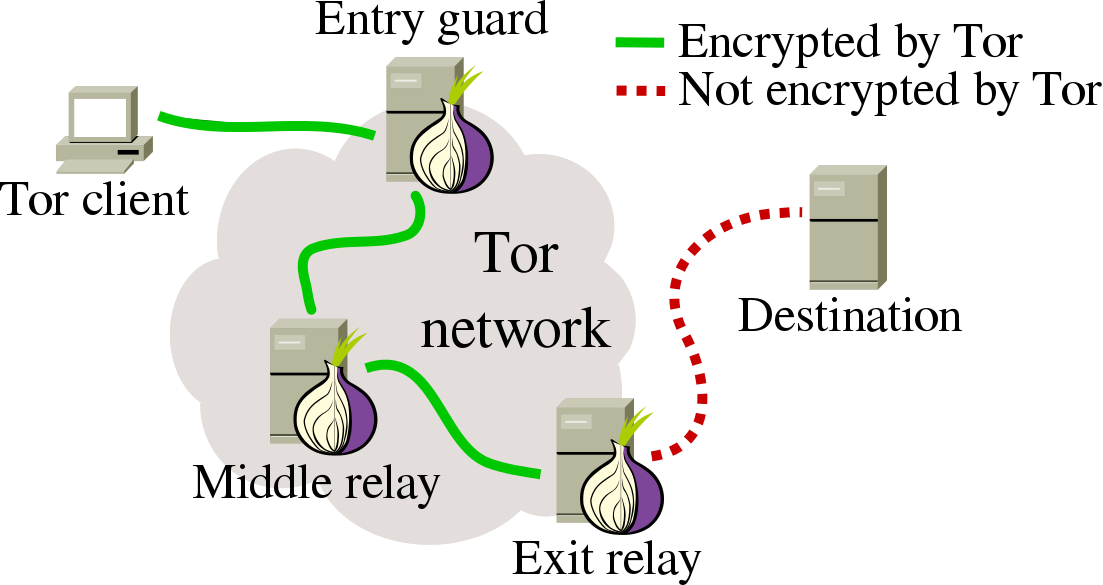
\includegraphics[width=\textwidth]{tor}
  \caption{Tor网络的主要组成部分,流量通过Tor网络的中继节点加密传输,在出口节点解密发送到目的地址。}
\end{figure}

本课题实现的多跳安全链路借鉴了Tor的思路,通过设置加密传输隧道的多个中继节点可以使攻击者难以确定加密流量的源IP地址,提高了匿名性和安全性。
同时,类似于Tor,每一个节点会对一层加密的数据进行解密,得到加密隧道的UUID来确定下一个节点,然后把数据转发到下一个节点。

\section{TLS}
传输层安全性协议(英语:Transport Layer Security,缩写:TLS)及其前身安全套接层(英语:Secure Sockets Layer,缩写:SSL)是一种安全协议,目的是为互联网通信提供安全及数据完整性保障。
网景公司(Netscape)在1994年推出首版网页浏览器-网景导航者时,推出HTTPS协议,以SSL进行加密,这是SSL的起源。
IETF将SSL进行标准化,1999年公布TLS 1.0标准文件(RFC 2246)。
随后又公布TLS 1.1(RFC 4346,2006年)、TLS 1.2(RFC 5246,2008年)和TLS 1.3(RFC 8446,2018年)。
该协议被广泛用于浏览器、电子邮件、即时通讯、VoIP、网络传真等应用中,但其在保障HTTPS方面的应用仍然是最广泛使用的。

\begin{figure}[H]
  \centering
  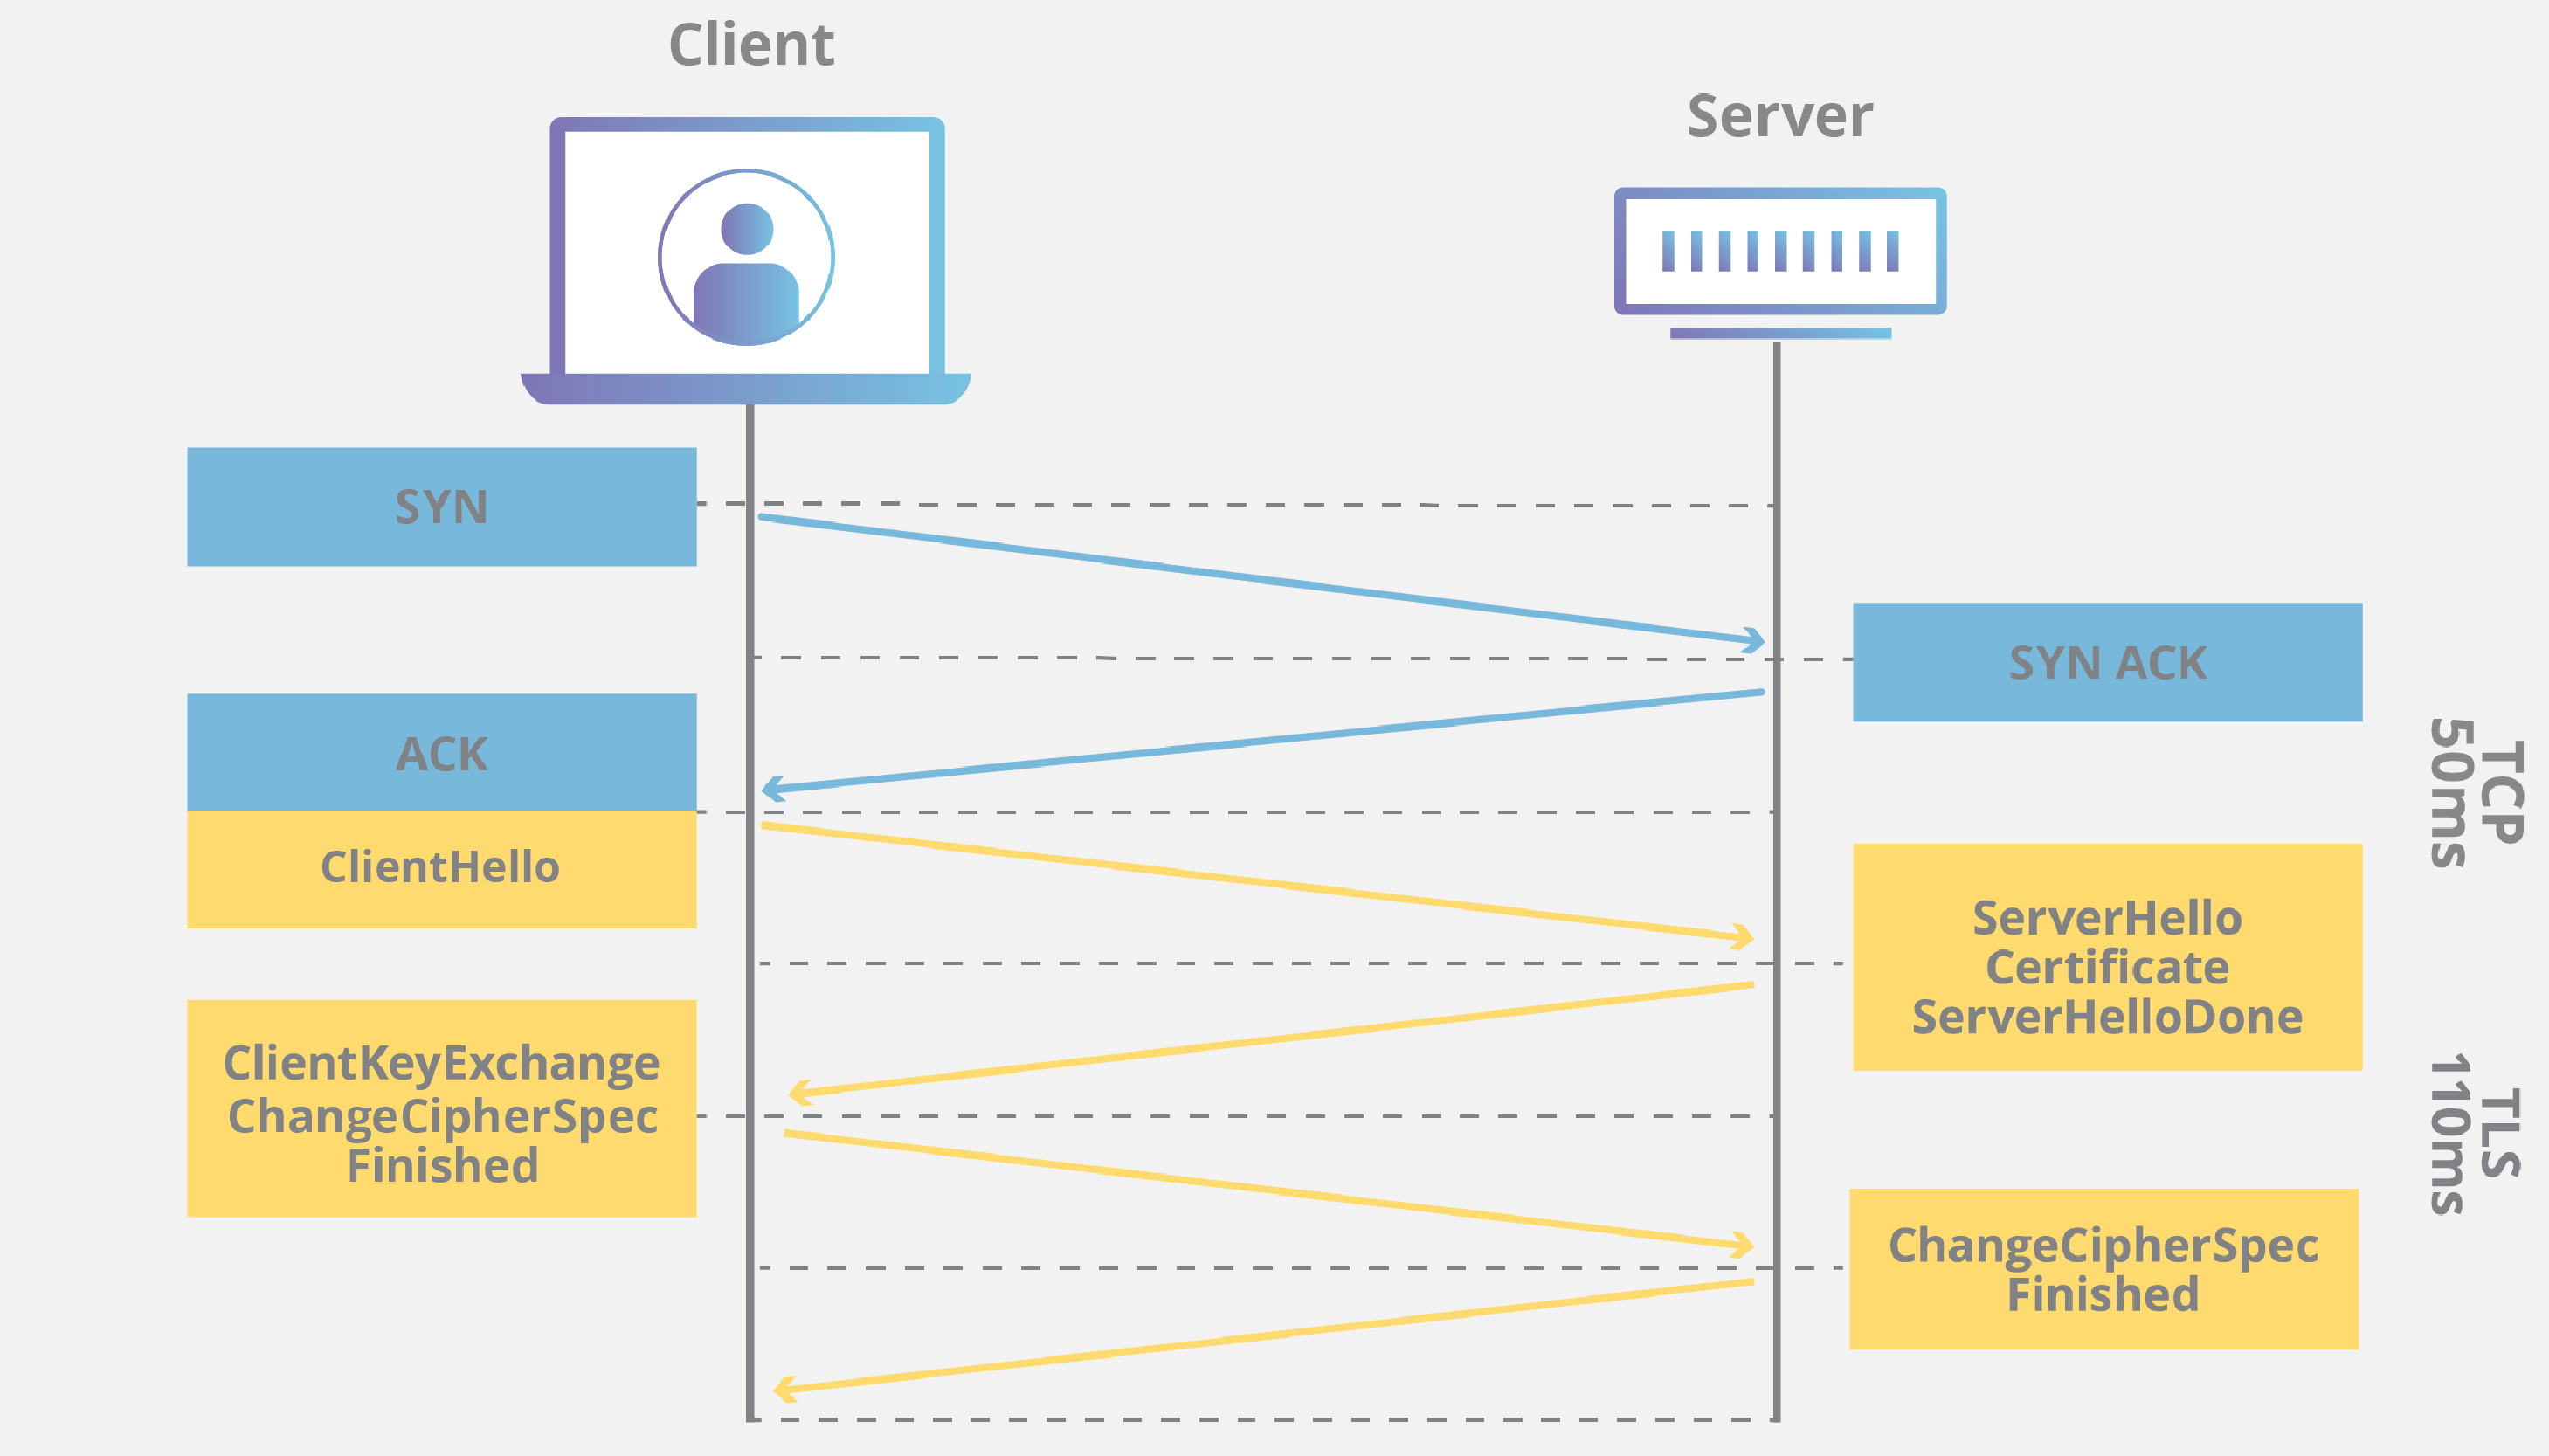
\includegraphics[width=\textwidth]{tls}
  \caption{TLS协议通信双方握手的过程}
\end{figure}

TLS协议包含以下几个基本阶段:
\begin{enumerate}
  \item 对等协商支持的TLS版本,和支持的密码包。
  \item 基于非对称密钥的身份认证,通常是基于PKI证书的身份认证。服务器将其X.509证书发送给客户端,由客户端验证服务器的身份。如果服务器要验证客户端的证书,则客户端可能会将客户端证书发送给服务器。通常仅验证服务器,不验证客户端。
  \item 基于对称密钥的数据加密。客户端生成随机数作为会话密钥,并使用服务器公钥(服务器公钥在服务器证书中)加密会话密钥,最后将已加密的会话密钥发送给服务器。由服务器的私钥解密出会话密钥。最后使用此会话密钥加密数据。TLS也可以使用预共享密钥(PSK)作为对称密钥。
\end{enumerate}

本课题实现的安全链路中,通过TLS协议来加密传输数据,TLS 1.3采用的AEAD加密算法,保证了认证加密(Authenticated encryption),这是一种能够同时保证数据的保密性、完整性和真实性的一种加密模式。
客户端和服务器在传输数据前先要经过密钥协商握手,之后双方通信的数据都经过共同协商的密钥加密传输。
TLS握手后,通信双方建立起一条安全的加密隧道。
由于采用流行的TLS协议,使得对流量的分析很困难,并且难以受到由于协议的特殊性导致的指纹攻击。

\section{SOCKS}
\begin{figure}[H]
  \centering
  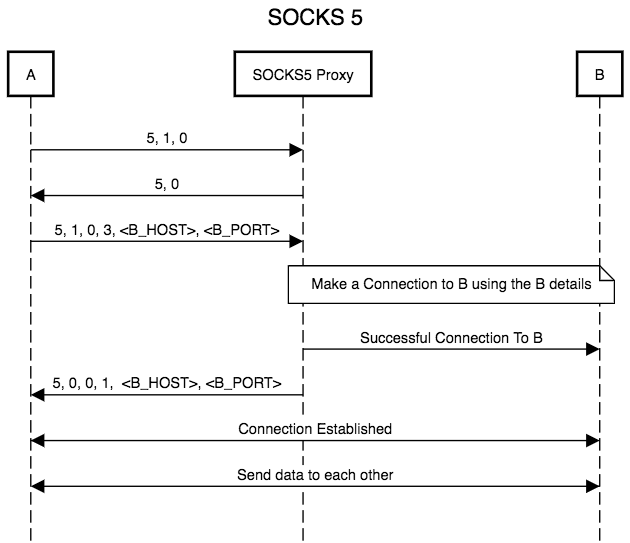
\includegraphics[width=\textwidth]{socks5}
  \caption{客户端通过SOCKS5代理服务器将请求发往外部的服务器}
\end{figure}

SOCKS是一种网络传输协议,处于OSI模型的会话层,主要用于客户端与外网服务器之间通讯的中间传递。
当防火墙后的客户端要访问外部的服务器时,就跟SOCKS代理服务器连接。这个代理服务器控制客户端访问外网的资格,允许的话,就将客户端的请求发往外部的服务器。
SOCKS工作在比HTTP代理更低的层次:SOCKS使用握手协议来通知代理软件其客户端试图进行的SOCKS连接,然后尽可能透明地进行操作,而常规代理可能会解释和重写报头(例如,使用另一种底层协议,例如FTP;然而,HTTP代理只是将HTTP请求转发到所需的HTTP服务器)。虽然HTTP代理有不同的使用模式,HTTP CONNECT方法允许转发TCP连接;然而,SOCKS代理还可以转发UDP流量(仅SOCKS5),而HTTP代理不能。

本课题实现了SOCKS5协议,这是SOCKS协议的最新版本。
这个新的版本扩展了SOCKS4,包括增加支持UDP,对该框架进行了扩展来包括对通用的强认证方案的规定,并将寻址方案扩展到涵盖了域名和IPV6地址。
用户设置代理为本地的SOCKS代理(默认在1080端口),就可以将用户流量通过客户端程序传输到加密隧道,最终到达目的服务器。